\section{一般同余子群的维数公式}
\label{sec:dim-general}
% ============================================================================

$\SL_2(\Z)$ 的公式虽然漂亮，但真正进入算术应用时，我们更常遇到的是 $\Gamma_0(N)$、$\Gamma_1(N)$ 一类带级别结构的群。此时空间维数不再只由一个“$k/12$”控制，而会受到三类几何数据共同影响：曲线的亏格 $g$、椭圆点个数 $\nu_2,\nu_3$，以及尖点个数 $\nu_\infty$。

直观地说，这些数据恰好记录了模曲线上最“异常”的点：亏格反映全局拓扑，椭圆点反映局部对称性，尖点反映无穷远处的退化。Riemann--Roch 把这三者合在一起，就给出了一条真正可计算的维数公式。

% figures/ch03-genus-vs-N.tex
% Bar chart for genus g(X_0(N)), N=1,...,20
\begin{figure}[ht]
\centering
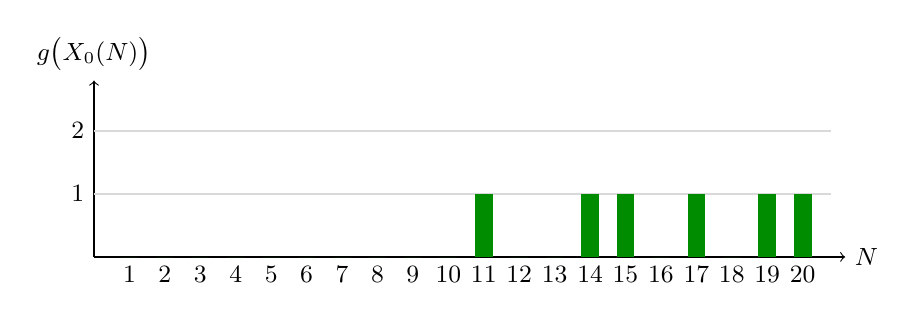
\begin{tikzpicture}[x=0.45cm,y=0.8cm,font=\small]
  \draw[->] (0,0) -- (21.2,0) node[right] {$N$};
  \draw[->] (0,0) -- (0,2.8) node[above] {$g\bigl(X_0(N)\bigr)$};

  \foreach \n in {1,...,20}
    \node[below] at (\n,0) {\n};
  \foreach \y in {1,2}
    {\draw[gray!30] (0,\y) -- (20.8,\y); \node[left] at (0,\y) {\y};}

  \foreach \n/\g in {1/0,2/0,3/0,4/0,5/0,6/0,7/0,8/0,9/0,10/0,11/1,12/0,13/0,14/1,15/1,16/0,17/1,18/0,19/1,20/1}
    \fill[green!55!black] (\n-0.25,0) rectangle (\n+0.25,\g);
\end{tikzpicture}
\caption{$X_0(N)$ 的亏格在小级别的分布。直到 $N=10$ 都还是亏格 $0$；从 $N=11$ 开始，权 $2$ cusp form 才真正稳定出现。}
\label{fig:genus-vs-N}
\end{figure}


为了避免 $\Gamma_1(N)$ 在不含 $-I$ 时出现的额外修正项，本节先陈述本书后续最常用、也是计算 $\Gamma_0(N)$ 时完全足够的版本：假设 $\Gamma$ 为有限指数同余子群，且 $-I\in \Gamma$。

\begin{theorem}[一般维数公式]
\label{thm:dim-general}
设 $\Gamma$ 为有限指数同余子群，满足 $-I\in\Gamma$。记
\[
  g=g\bigl(X(\Gamma)\bigr),\qquad \nu_2=\#\{\text{阶 }2\text{ 椭圆点}\},
  \qquad \nu_3=\#\{\text{阶 }3\text{ 椭圆点}\},
  \qquad \nu_\infty=\#\{\text{尖点}\}.
\]
则对偶数权 $k\ge 2$，有
\[
  \dim \Mk_k(\Gamma)
  =(k-1)(g-1)+\left\lfloor\frac{k}{4}\right\rfloor\nu_2
   +\left\lfloor\frac{k}{3}\right\rfloor\nu_3
   +\frac{k}{2}\nu_\infty,
\]
并且对偶数权 $k\ge 4$，有
\[
  \dim \Sk_k(\Gamma)
  =(k-1)(g-1)+\left\lfloor\frac{k}{4}\right\rfloor\nu_2
   +\left\lfloor\frac{k}{3}\right\rfloor\nu_3
   +\left(\frac{k}{2}-1\right)\nu_\infty.
\]
在 $k=2$ 时，特殊情形为
\[
  \dim \Sk_2(\Gamma)=g,
\]
与上一章得到的结果一致。
\end{theorem}

\begin{example}[$\Gamma_0(11)$：第一个亏格 $1$ 的例子]
\label{ex:dim-gamma0-11}
对 $\Gamma_0(11)$，有
\[
  \mu=[\SL_2(\Z):\Gamma_0(11)]=11\left(1+\frac1{11}\right)=12,
\]
且
\[
  \nu_2=0,\qquad \nu_3=0,\qquad \nu_\infty=2.
\]
故由上一章的 genus formula，
\[
  g=1+\frac{12}{12}-0-0-\frac22=1.
\]
于是
\[
  \dim \Sk_2(\Gamma_0(11))=g=1.
\]
这就是那条熟悉的新形式
\[
  f=q-2q^2-q^3+2q^4+q^5+\cdots
\]
出现且唯一的原因。再算一个更高权例子：当 $k=12$ 时，
\[
  \dim \Sk_{12}(\Gamma_0(11))
  =11\cdot 0+0+0+\left(6-1\right)\cdot 2=10.
\]
所以级别一旦升高，空间维数增长得会比全模群快得多。
\end{example}

\begin{proof}[证明思路]
这是 Riemann--Roch 在线丛 $\mathcal L^{k/2}$ 上的直接应用。大致步骤如下：
\begin{enumerate}
  \item 把 $\Mk_k(\Gamma)$ 识别为模曲线 $X(\Gamma)$ 上某个除子 $D_k$ 的截面空间 $L(D_k)$；
  \item 在阶 $2$、阶 $3$ 椭圆点处分别使用平方、立方局部参数，在尖点处使用 $q_h=e^{2\pi i\tau/h}$，就会得到
        $\lfloor k/4\rfloor\nu_2$、$\lfloor k/3\rfloor\nu_3$ 和 $(k/2)\nu_\infty$ 这些局部贡献；
  \item 对 cusp form，只需在每个尖点再要求多消失一次，于是尖点项从 $(k/2)\nu_\infty$ 变成
        $\left(\frac{k}{2}-1\right)\nu_\infty$；
  \item 当 $k\ge 2$ 时，相关除子已足够大，Riemann--Roch 中的余项 $\ell(K-D_k)$ 消失；把剩下的“次数减亏格加一”整理后，就正好得到定理中的公式。
\end{enumerate}
完整证明涉及椭圆点和尖点的局部坐标核算，见 Diamond--Shurman, §3.6。
\end{proof}

\begin{proposition}[$\Gamma_0(N)$ 的几何输入量]
\label{prop:gamma0N-ingredients}
对 $\Gamma_0(N)$，上面公式中的几何量可以显式写成：
\begin{align*}
  \mu&=[\SL_2(\Z):\Gamma_0(N)]=N\prod_{p\mid N}\left(1+\frac1p\right),\\
  \nu_2&=\#\{c\bmod N: c^2\equiv -1\pmod N\},\qquad (\text{若 }4\mid N\text{ 则 }\nu_2=0),\\
  \nu_3&=\#\{c\bmod N: c^2+c+1\equiv 0\pmod N\},\qquad (\text{若 }9\mid N\text{ 则 }\nu_3=0),\\
  \nu_\infty&=\sum_{d\mid N}\varphi\bigl(\gcd(d,N/d)\bigr),\\
  g\bigl(X_0(N)\bigr)&=1+\frac{\mu}{12}-\frac{\nu_2}{4}-\frac{\nu_3}{3}-\frac{\nu_\infty}{2}.
\end{align*}
\end{proposition}

\begin{example}[$\Gamma_0(37)$ 与 $\Gamma_0(1)$]
\label{ex:gamma0-37-and-1}
\begin{enumerate}
  \item 对 $N=37$，有
        \[
          \mu=37\left(1+\frac1{37}\right)=38,
          \qquad \nu_2=0,
          \qquad \nu_3=0,
          \qquad \nu_\infty=2.
        \]
        因而
        \[
          g\bigl(X_0(37)\bigr)=1+\frac{38}{12}-1=2.
        \]
        所以
        \[
          \dim \Sk_2(\Gamma_0(37))=2.
        \]
        这说明在级别 $37$、权 $2$ 时，Hecke 算子已经需要在一个二维空间里对角化。

  \item 当 $N=1$ 时，$\Gamma_0(1)=\SL_2(\Z)$，并且
        \[
          g=0,\qquad \nu_2=1,\qquad \nu_3=1,\qquad \nu_\infty=1.
        \]
        代入一般公式可得
        \[
          \dim \Mk_k(\SL_2(\Z))=-(k-1)+\left\lfloor\frac{k}{4}\right\rfloor+
          \left\lfloor\frac{k}{3}\right\rfloor+\frac{k}{2}.
        \]
        对偶数 $k$ 分六个模 $12$ 的余类检查，正好化简成
        \[
          \dim \Mk_k(\SL_2(\Z))=
          \begin{cases}
            \lfloor k/12\rfloor+1,& k\not\equiv 2\pmod{12},\\
            \lfloor k/12\rfloor,& k\equiv 2\pmod{12},
          \end{cases}
        \]
        也就是上一节的公式。
\end{enumerate}
\end{example}

下面给出小级别的一张常用表。它很适合快速判断“这个级别是否已经可能出现权 $2$ cusp form”。

\begin{center}
\begin{tabular}{c|cccccccccccc}
\toprule
$N$ & 1 & 2 & 3 & 4 & 5 & 6 & 7 & 8 & 9 & 10 & 11 & 12 \\
\midrule
$g\bigl(X_0(N)\bigr)$ & 0 & 0 & 0 & 0 & 0 & 0 & 0 & 0 & 0 & 0 & 1 & 0 \\
$\nu_2$ & 1 & 1 & 0 & 0 & 2 & 0 & 0 & 0 & 0 & 2 & 0 & 0 \\
$\nu_3$ & 1 & 0 & 1 & 0 & 0 & 0 & 2 & 0 & 0 & 0 & 0 & 0 \\
$\nu_\infty$ & 1 & 2 & 2 & 3 & 2 & 4 & 2 & 4 & 4 & 4 & 2 & 6 \\
\bottomrule
\end{tabular}
\end{center}

\begin{proposition}[权 $2$ 的完整小级别表]
\label{prop:dim-s2-table-50}
对 $\Gamma_0(N)$，有
\[
  \dim \Sk_2(\GammaO(N))=g\bigl(X_0(N)\bigr).
\]
因此利用上一章的 genus formula，可以把 $N=1$ 到 $50$ 的数值完全列出如下。
\end{proposition}

\begin{center}
\small
\begin{longtable}{@{}cccc@{}}
\toprule
$N$ & $\dim \Sk_2(\GammaO(N))$ & $N$ & $\dim \Sk_2(\GammaO(N))$ \\
\midrule
\endfirsthead
\toprule
$N$ & $\dim \Sk_2(\GammaO(N))$ & $N$ & $\dim \Sk_2(\GammaO(N))$ \\
\midrule
\endhead
1 & 0 & 26 & 2 \\
2 & 0 & 27 & 1 \\
3 & 0 & 28 & 2 \\
4 & 0 & 29 & 2 \\
5 & 0 & 30 & 3 \\
6 & 0 & 31 & 2 \\
7 & 0 & 32 & 1 \\
8 & 0 & 33 & 3 \\
9 & 0 & 34 & 3 \\
10 & 0 & 35 & 3 \\
11 & 1 & 36 & 1 \\
12 & 0 & 37 & 2 \\
13 & 0 & 38 & 4 \\
14 & 1 & 39 & 3 \\
15 & 1 & 40 & 3 \\
16 & 0 & 41 & 3 \\
17 & 1 & 42 & 5 \\
18 & 0 & 43 & 3 \\
19 & 1 & 44 & 4 \\
20 & 1 & 45 & 3 \\
21 & 1 & 46 & 5 \\
22 & 2 & 47 & 4 \\
23 & 2 & 48 & 3 \\
24 & 1 & 49 & 1 \\
25 & 0 & 50 & 2 \\
\bottomrule
\end{longtable}
\normalsize
\end{center}

从这张表里立刻可以读出两条最常用的信息：
\begin{align*}
  \dim \Sk_2(\GammaO(N))=0
  &\Longleftrightarrow
  N\in\{1,2,3,4,5,6,7,8,9,10,12,13,16,18,25\},\\
  \dim \Sk_2(\GammaO(N))=1
  &\Longleftrightarrow
  N\in\{11,14,15,17,19,20,21,24,27,32,36,49\}.
\end{align*}
第一行恰好是小级别里 $X_0(N)\cong \mathbb P^1$ 的列表；
第二行说明这些级别上最小的非平凡模 Abel 簇已经是一条椭圆曲线。
特别地，$N=11$ 是第一条真正出现模椭圆曲线的级别。

\textbf{与 FLT 的直接联系。}
在 Wiles--Ribet 的证明链条里，
Frey 曲线的 residual 表示经过水平下降会被逼到级别 $2$。
而表中第 $N=2$ 行明确告诉我们
\[
  \dim \Sk_2(\GammaO(2))=0.
\]
这意味着级别 $2$ 根本不存在权 $2$ 新形式，
也就不存在能够承载那份 residual 特征值系统的模 Jacobian 因子。
因此“降到 $X_0(2)$”并不是一句口号，
而是把矛盾压缩成一条具体的维数等式：
$X_0(2)$ 是亏格 $0$ 曲线，所以没有权 $2$ cusp form。

\begin{remark}[关于 $\Gamma_1(N)$]
当 $N>2$ 时，$\Gamma_1(N)$ 往往不含 $-I$，于是奇偶权与尖点局部行为会带来额外修正项。其完整公式仍然来自同样的 Riemann--Roch 机制，只是记号更繁。就本书后续讨论 Hecke 新形式与模性问题而言，最核心、最常用的版本正是上面的 $\Gamma_0(N)$ 公式。
\end{remark}
